\section{Definition of a battery model}

In order to define a good model for Li-Po battery, comprehending also a good approximation of all its non-idealities, a two-branches model has been used.
In the first part, current SoC is computed, by taking as a reference electrical model a current generator and a capacitor. The discharge current $I_{b}$ charges the capacitor, of capacity $C_{m}$ (representing the total capacity of the battery), producing an output voltage $V_{SOC}$ which represents the SoC. 


The output equation of the circuit is thus $V_{SOC} = V_{SOC}(0)+\int\!\frac{I_{b}}{C_{m}}dt$, which is equivalent to the SoC expression for the battery.

The second part of the model is composed by a voltage generator and a series resistance, as in a usual models of voltage sources. The big difference from standard models is that both the voltage and the series resistance of the battery depend on the current state of charge, and are thus functions of $V_{SOC}$.

The output of this second circuit is the true battery voltage as seen by the load.

\begin{figure}[h]
  \centering
  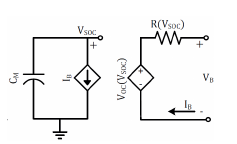
\includegraphics[width=3in]{circuit}
  \caption{Equivalent circuit of the Li-Po battery}
\end{figure}

While the first part of the circuit is well-defined by the initial and total capacity of the battery, in the second part the two functions $V(SoC)$ and $R(SoC)$ has to be extracted from available battery data. In this case, the available source of information contained into the battery's datasheet has been the graph showing output voltage ($V_{B}$) as a function of both discharge capacity - which is, after fixing a maximum capacity value, easily convertible to SoC - and load current. The latter dependance is due to the series resistance of the battery.

Points from these curves have been extracted using a figure digitizer tool into MatLab and have been converted to different Soc-voltage tables. In order to find a good value for R two curves have been necessary (as R affects only the $V_{B}$-$I_{load}$ relationship). To minimize sampling errors, the highest and lowest currents' curves have been digitalized. Finally, the saved data have been interpolated in a linear fashion to obtain a continous sequence of equally-spaced points on the graph.

From these data, $V(Soc)$ and $R(Soc)$ values can be easily obtained by solving the second circuit. Although at this point a model of the two circuits has been made, having the values stored as a lookup table is not the best choice, both because of the space occupation which would not scale for bigger graphs, and because of the missing smoothness of the obtained relationship, which is typical of a real-life system. In order to obtain a smoother and simpler relationship, the data have been fitted using MatLab $fmins$ function, in order to have an analytical representation for them:
\begin{align*}
V(SoC)&=b_1e^{(b_2SoC)}+b_3SoC^4+b_4SoC^3+b_5SoC^2+b_6SoC+b_7 \\
R(SoC)&=b_8e^{(b_9SoC)}+b_{10}
\end{align*}

The curve fitting produced a satisfactory result:

\begin{center}
\begin{tabular}{|c| c|}

    \hline
    Parameter name & Parameter value \\
    \hline
    $b_{1}$ & 1.3518 \\
    $b_{2}$ & -0.7752 \\
    $b_{3}$ & 0.4669 \\
    $b_{4}$ & -1.0723 \\
    $b_{5}$ & 0.8729 \\
    $b_{6}$ & -0.0031 \\
    $b_{7}$ & 2.8434 \\
    $b_{8}$ & 0.0000 \\
    $b_{9}$ & 9.7875 \\
    $b_{1}$ & 0.1909 \\
    \hline
\end{tabular}


\begin{figure}[h]
  \centering
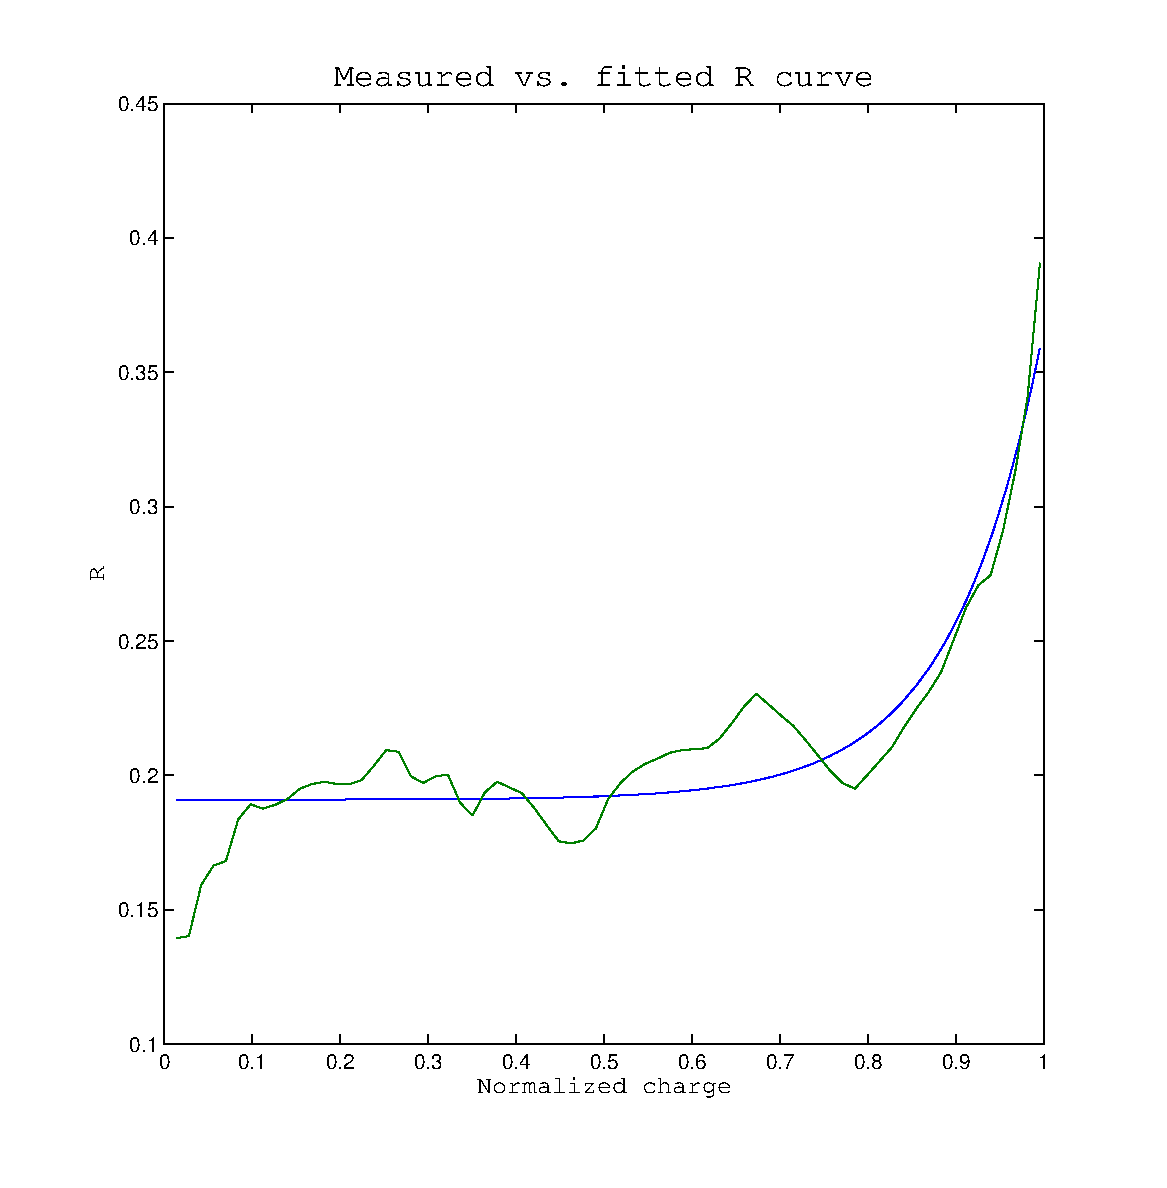
\includegraphics[width=3in]{fitted_r_curve}
\caption{$SoC-R$ curve after fitting}
\end{figure}


\begin{figure}[h]
  \centering
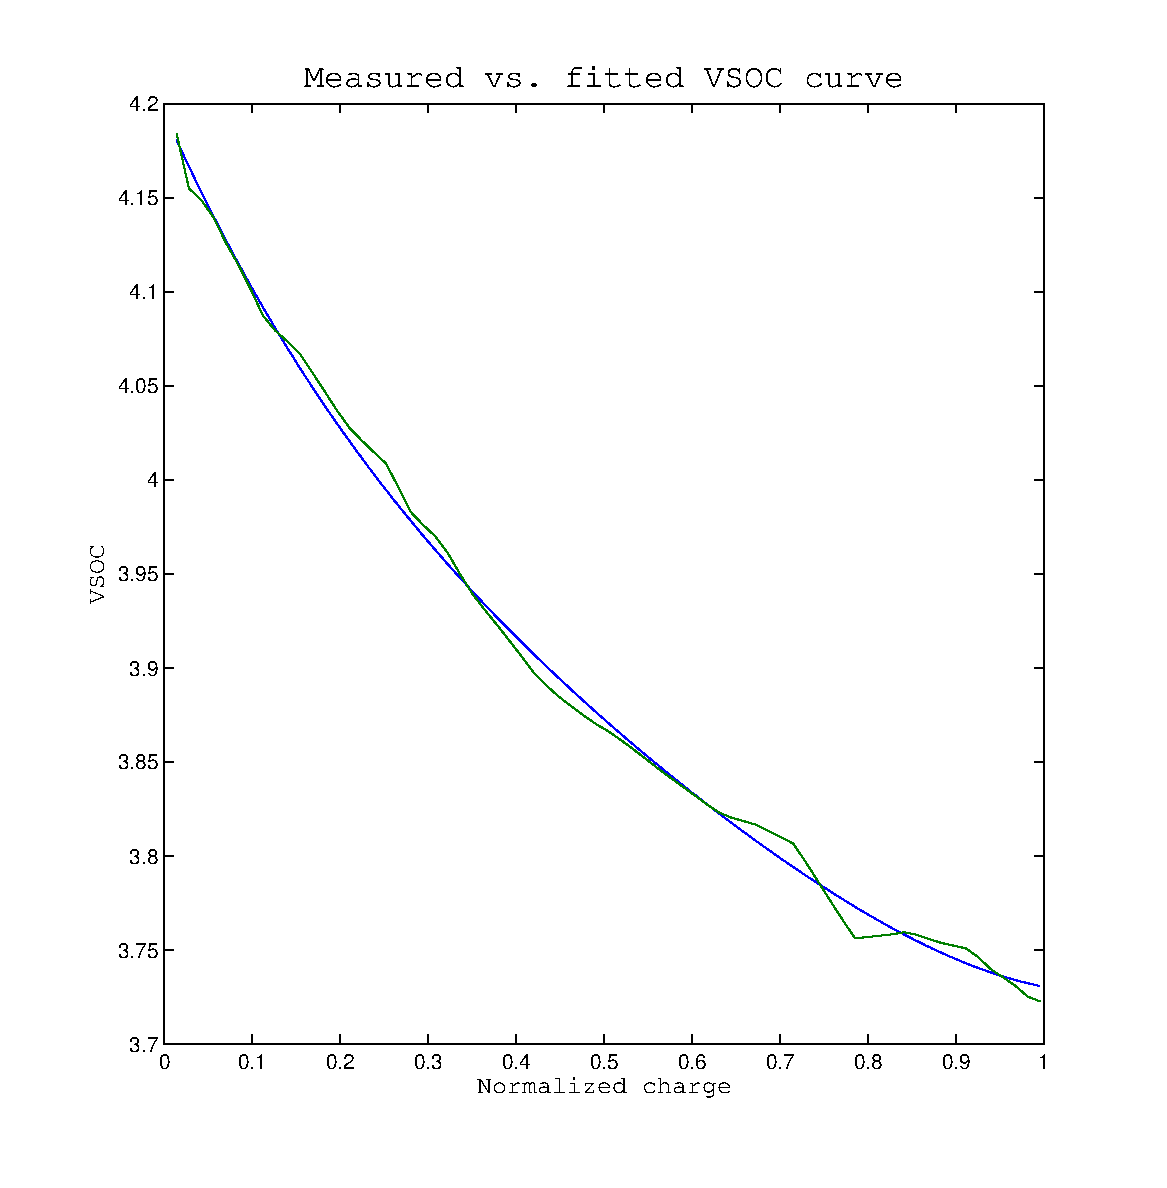
\includegraphics[width=4in]{fitted_vsoc_curve} 
\caption{$SoC-V$ curve after fitting}
\end{figure}

\end{center}


